\chapter{\mysketch}
\label{chap:quancurrent}

We present \mysketch, an $r$-relaxed concurrent Quantiles sketch where $r$ depends on system parameters as discussed below. The algorithm uses $N$ update threads to ingest stream elements and allows an unbounded number of query threads. Queries are processed at any time during the sketch's construction. 
We consider a shared memory model that provides synchronization variables (atomics) and atomic operations to guarantee sequential consistency as in C++~\cite{Boehm_2008_cpp}. Everything that happened-before a write in one thread becomes visible to a thread that reads the written value. Also, there is a single total order in which all threads observe all modification in the same order. 
We use the following sequentially consistent atomic operations (which force a full fence): \emph{fetch-and-add (F\&A)}~\cite{x86-faa} and \emph{compare-and-swap (CAS)}~\cite{x86-cas}. 

In addition, we use a software-implemented higher-level primitive, \emph{double-compare-double-swap (DCAS)} which atomically updates two memory addresses as follows: DCAS($addr_1$: $old_1 \to new_1$, $addr_2$: $old_2 \to new_2$)
is given two memory addresses $addr_1$, $addr_2$, two corresponding expected values $old_1$, $old_2$, and two new values $new_1$, $new_2$ as arguments. It atomically sets $addr_1$ to $new_1$ and $addr_2$ to $new_2$ only if both addresses match their expected values, i.e., the value at $addr_1$ equals $old_1$ and the value at $addr_2$ equals $old_2$. DCAS also provides wait-free DCAS\_READ primitive, which can read fields that are concurrently modified by a DCAS. DCAS can be efficiently implemented using single-word CAS~\cite{Harris2002practical,guerraoui2020efficient}. 


In Section~\ref{sec:data_org}, we present the data structures used by Quancurrent. Section~\ref{sec:update_alg} presents the update operation, and \todo[color=red]{fix} Section~\ref{sec:query_alg} presents the query. The formal correctness proof is deferred to the supplementary material. 

%============================================================
\section{Data Structures} \label{sec:data_org}
%============================================================
\mysketch's data structures are described in Algorithm~\ref{alg:data_organization} and depicted in Figure~\ref{fig: data_structures}.
Similarly to the sequential Quantiles sketch, \mysketch is organized as a hierarchy of arrays called \emph{levels}. Each level can be \emph{empty}, \emph{full}, or in \emph{propagation}. The variable \emph{tritmap} maintains the states of all levels. Tritmap is an unsigned integer, interpreted as an array of trits (trinary digits). The trit $tritmap[i]$ describes level $i$'s state: if $tritmap[i]$ is $0$, level $i$ contains $0$ or $2k$ ignored elements and is considered to be empty. If $tritmap[i]$ is $1$, level $i$ contains $k$ elements and is deemed full, and if it is $2$, level $i$ contains $2k$ elements and is associated with the propagation state. Each thread has a local buffer of size $b$, $\mathit{localBuf[b]}$. Before ingested into the sketch's levels, stream elements are buffered in threads local buffers and then moved to a processing unit called $\mathit{Gather\&Sort}$. The $\mathit{Gather\&Sort}$ object has two $2k$-sized shared buffers, $\mathit{G\&SBuffer}[2]$, each with its own $\mathit{index}$ specifying the current location, as depicted in Figure~\ref{fig: gather_and_sort}. 

The query mechanism of \mysketch includes taking an atomic snapshot of the levels. Query threads cache the snapshot and the tritmap that represents it in local variables, 
$\mathit{snapshot}$ and $\mathit{myTrit}$, respectively. As the snapshot reflects only the sketch's levels and not G\&SBuffers or the thread's local buffers, Quancurrent is ($4kS+(N-S)b$)-relaxed Quantiles sketch where $S$ is the number of NUMA nodes. 


\begin{algorithm}[h]
\caption{\mysketch data structures} \label{alg:data_organization}
    \begin{algorithmic}[1] 
    \setcounter{ALG@line}{\value{mycounter}}
    \State \textbf{Parameters and constants:}
        \State \hspace{\algorithmicindent} \myvar{MAX\_LEVEL} 
        \State \hspace{\algorithmicindent} \myvar{k} \Comment{sketch level size}
        \State \hspace{\algorithmicindent} \myvar{b} \Comment{local buffer size}
        \State \hspace{\algorithmicindent} \myvar{S} \Comment{\#NUMA nodes}
    \State
    \State \textbf{Shared objects:} \;
        \State \hspace{\algorithmicindent} \myvar{tritmap} $\gets 0$ 
        \State \hspace{\algorithmicindent} \myvar{levels}[\myvar{MAX\_LEVEL}]
    \State
    \State \textbf{NUMA-local objects:} \Comment{shared among threads on the same node}
        \State \hspace{\algorithmicindent} \myvar{G\&SBuffer}[2][2\myvar{k}]
        \State \hspace{\algorithmicindent} \myvar{index}[2] $\gets \{0,0\}$
    \State
    \State \textbf{Thread local objects:}
        \State \hspace{\algorithmicindent} \myvar{localBuf}[\myvar{b}]
        \State \hspace{\algorithmicindent} \myvar{myTrit} \Comment{used by query}
        \State \hspace{\algorithmicindent} \myvar{snapshot} \Comment{used by query}
        \setcounter{mycounter}{\value{ALG@line}}
    \end{algorithmic}
\end{algorithm}

%============================================================
\section{Update} \label{sec:update_alg} %Blocking, Holes, Double Base Buffer, Sorted Local Buffers Update, Merge using k-Way Merge Sort
%============================================================
The ingestion of stream elements occurs in three stages: 
(1) \emph{gather and sort}, 
(2) \emph{batch update}, and 
(3) \emph{propagate level}. 
In stage (1), stream elements are buffered and sorted into batches of $2k$ through a $\mathit{Gather\&Sort}$ object. Each NUMA node has its designated $\mathit{Gather\&Sort}$ object, which is accessed by NUMA-local threads. 
Stage (2) executes a batch update of $2k$ elements from the $\mathit{Gather\&Sort}$ object to $levels[0]$. 
Finally, in stage (3), $levels[0]$ is propagated up the levels of the hierarchy.

%============================================================
% \subsubsection{Stage 1: Gather and Sort} \label{Section: part1_update} 
%============================================================
In the first stage, threads first process stream elements into a thread-local buffer of size $b$. Once the buffer is full, it is sorted and the thread reserves $b$ slots on a shared buffer in its node's Gather\&Sort unit. It then begins to move the local buffer's content to the shared buffer. The shared Gather\&Sort buffer contains $2k$ elements, and its propagation (during Stage 2) is not synchronized with the insertion of elements. Thus, some reserved slots might still contain old values, (which have already been propagated), instead of new ones. As the batch is a sample of the original stream, we can accept the possible loss of information in order to improve performances. Below, we show that the sampling bias this introduces is negligible.

The pseudo-code for the first stage is presented in Algorithm~\ref{alg:gather}. To insert its elements to the shared buffer, a thread tries to reserve $b$ places in one of the shared buffers using F\&A (Line~\ref{Line: fetch_idx}). If the index does not overflow, the thread copies its local buffer to the reserved slots (Line~\ref{Line: copy_local_buffer}). We refer to the thread that fills the last $b$ locations in a G\&SBuffer as the \emph{owner} of the current batch. The batch owner creates a local sorted copy of the shared buffer and begins its propagation (Lines~\ref{Line:create_copy}-\ref{Line:call_batchUpdate}).

Note that the local buffer is not atomically moved into the shared buffer (Line \ref{Line: copy_local_buffer} is a loop). Thus, the owner might begin a propagation before another thread has finished moving its elements to the shared buffer. In this case, the old elements already contained within the G\&SBuffer are taken instead. Furthermore, upon moving its elements later, the writer thread might overwrite more recent elements. In other words, during this stage, stream elements may be duplicated and new elements may be dropped. We call both of these occurrences \emph{holes}, and analyze their implications in Section~\ref{ssec:holes-analysis} \todo[color=red]{fix}.


\begin{algorithm}[h]
\caption{Stage 1: gather and sort} \label{alg:gather}
% \alglanguage{algpseudocode}
\begin{algorithmic}[1]
\setcounter{ALG@line}{\value{mycounter}}
\Procedure{update}{$x$}
    \State add $\mathit{x}$ to \myvar{localBuf} \Comment{thread-local} \label{Line: update_linearization}
    \If{$\neg \mathit{localBuf}$.full()}
        \State \Return
    \EndIf
    \State sort \myvar{localBuf}
    \State \myvar{i} $\gets 0$
    \While{\textbf{true}} \Comment{insert to Gather\&Sort unit}
        \State \myvar{idx} $\gets$ \myvar{index}[\myvar{i}].F\&A(\myvar{b}) \label{Line: fetch_idx}
        \If{$\mathit{idx}< 2k$}
            \State move \myvar{localBuf} to \myvar{G\&SBuffer}[\myvar{i}][$\mathit{idx}, \dots, \mathit{idx}+b$] \label{Line: copy_local_buffer}
            \If{$\var{idx}+b=2k$} \Comment{owner, filled buffer}
                \State $\mathit{myCopy} \gets \text{sorted copy of } \mathit{G\&SBuffer}[\mathit{i}]$ \label{Line:create_copy}
                \State batchUpdate(\myvar{i},\myvar{myCopy}) \label{Line:call_batchUpdate}
            \EndIf
            \State \Return
        \EndIf
        \State \myvar{i} $\gets$ $\neg$\myvar{i}
    \EndWhile
\EndProcedure
\setcounter{mycounter}{\value{ALG@line}}
\end{algorithmic}
\end{algorithm}



\begin{figure}[h]
    \begin{subfigure}[b]{\linewidth}
    \centering
    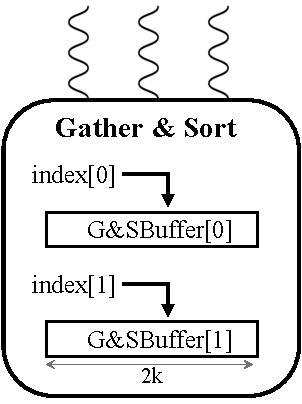
\includegraphics[width=0.3\linewidth]{graphics/algorithm/gather_and_sort.pdf}
    \caption{$\mathit{Gather\&Sort}$ object.}
    \label{fig: gather_and_sort}
    \end{subfigure}
    % \vfill
    \par\medskip
    \begin{subfigure}[b]{\linewidth}
    \centering
    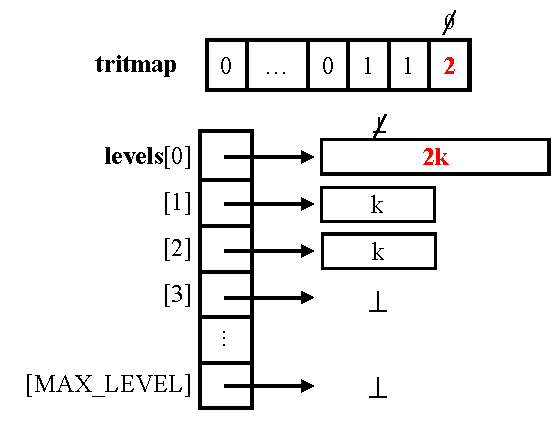
\includegraphics[width=0.5\linewidth]{graphics/algorithm/batch_update.pdf}
    \caption{Batch update into $\mathit{levels}[0]$.}
    \label{fig: batch_update}
    \end{subfigure}%
    
    \caption{Quancurrent's data structures.}
    \label{fig: data_structures}
\end{figure}




%============================================================
% \subsubsection{Stage 2: Batch Update} \label{Section: part2_batch_update}
%============================================================
In the second stage, the owner inserts its local sorted copy of the shared buffer into level $0$ using a DCAS. The batch of $2k$ elements is only inserted when level $0$ is empty, reflected by the first digit of the tritmap being $0$. We use DCAS to atomically update both \emph{levels}[0] to point to the new sorted batch and \emph{tritmap} to indicate an ongoing batch update (reflected by setting $\mathit{tritmap[0]}$ to 2). The DCAS might fail if other owner threads are trying to insert their batches or propagate them. The owner keeps trying to insert its batch into the sketch's first level until a DCAS succeeds, and then resets the index of the G\&SBuffer to allow other threads to ingest new stream elements. 
The pseudo-code for the second stage is presented in Algorithm~\ref{alg: batch_update}, and an example is depicted in Figure~\ref{fig: batch_update}.

\begin{algorithm}
\caption{Stage 2: batch update} \label{alg: batch_update}
\begin{algorithmic}[1]
\setcounter{ALG@line}{\value{mycounter}}
\Procedure{batchUpdate}{\myvar{i},\myvar{base\_copy}}
    \While{$\neg$DCAS(\myvar{levels}[0]: $\bot \to$ \myvar{base\_copy}, \myvar{tritmap}[0]: 0 $\to$ 2} \label{Line:insert_batch}
        \State \myvar{index}[\myvar{i}] $\gets 0$
        \State propagate(0)
    \EndWhile
\EndProcedure
\setcounter{mycounter}{\value{ALG@line}}
\end{algorithmic}
\end{algorithm}


%============================================================
% \subsubsection{Stage 3: Propagate Level} \label{Section: part3_propagate} 
%============================================================
In the beginning of the third stage, level 0 points to a new sorted copy of a \emph{G\&SBuffer} array and \emph{tritmap}[0]=2. During this stage, the owner thread propagates the newly inserted elements up the levels hierarchy iteratively, level by level from level 0 until an empty level is reached. The pseudo-code for the propagation stage is presented in Algorithm~\ref{alg: propagate}. On each call to \emph{propagate}, level $l$ is propagated to level $l+1$, assuming that level $l$ contains $2k$ sorted elements and $\mathit{tritmap}[l]=2$. If $\mathit{tritmap}[l+1]=2$, the owner thread is blocked by another propagation from $l+1$ to $l+2$ and it waits until $\mathit{tritmap}[l+1]$ is either a $0$ or $1$. The owner thread samples $k$ elements from level $l$ and retains the odd or even elements with equal probability (Line~\ref{Line: choose_rand}). 
If $\mathit{tritmap}[l+1]$ is $1$, then level $l+1$ contains $k$ elements. The sampled elements are merged with level $l$+1 elements into a new $2k$-sized sorted array (Line~\ref{Line: next_full}). We then (in Line~\ref{Line:next_full_DCAS}) continuously try, using DCAS, to update \emph{levels}[$l$+1] to point to the merged array and atomically update \emph{tritmap} such that \emph{tritmap}[$l$] $\gets 0$, reflecting level $l$ is available, and \emph{tritmap}[$l$+1] $\gets 2$, reflecting that level $l$+1 contains $2k$ elements. After a successful DCAS, we clear level $l$ (set it to $\bot$) and proceed to propagate the next level (Line~\ref{Line:propagate_next}). 
If $\mathit{tritmap}[l+1]$ is $0$, then level $l+1$ is empty. We use DCAS (Line~\ref{Line:next_empty_DCAS}) to update $\mathit{levels}[l+1]$ to point to the sampled elements and atomically update \emph{tritmap} so that \emph{tritmap}[$l$] becomes $0$, and \emph{tritmap}[$l$+1] becomes $1$ (containing $k$ elements). After a successful DCAS, we clear level $l$ (set it to $\bot$) and end the current propagation.

Propagations of different batches may occur concurrently, i.e., level propagation of levels $l$ and $l'$ can be performed in parallel. Figure~\ref{fig: propagate} depicts an example of concurrent propagation of two batches.


\begin{algorithm}[h]
\caption{Stage 3: Propagation of level $l$} \label{alg: propagate}
\begin{algorithmic}[1]
\setcounter{ALG@line}{\value{mycounter}}
\Procedure{propagate}{\myvar{l}}
    \If{ \myvar{l} $\geq$ \myvar{MAX\_LEVEL} }
        \State \Return
    \EndIf
    \State \myvar{newLevel} $\gets$ sampleOddOrEven(\myvar{levels}[\myvar{l}]) \Comment{choose odd or even indexed elements randomly} \label{Line: choose_rand}
    \If{\myvar{tritmap}[\myvar{l}$+1$] $ =1$} \Comment{next level is full}
        \State \myvar{newLevel} $\gets$ merge(\myvar{newLevel}, \myvar{levels}[\myvar{l}$+1$]) \label{Line: next_full}
        \While{$\neg$DCAS(\myvar{levels}[\myvar{l}$+1$]: \myvar{levels}[\myvar{l}$+1$] $\to$ \myvar{newLevel},  \myvar{tritmap}[\myvar{l}, \myvar{l}$+1$]: $ [2,1] \to [0,2]$)} \{\} \label{Line:next_full_DCAS}
        \EndWhile
        \State \myvar{levels}[\myvar{l}] $\gets \bot$ \Comment{clear level} 
        \State \Return{propagate(\myvar{l}+1)} \label{Line:propagate_next}
    \EndIf
    \While{$\neg$DCAS(\myvar{levels}[\myvar{l}$+1$]: $ \bot \to$ \myvar{newLevel}, \myvar{tritmap}[\myvar{l}, \myvar{l}$+1$]: $ [2,0] \to [0,1]$)} \{\} \label{Line:next_empty_DCAS}
    \EndWhile
    \State \myvar{levels}[\myvar{l}] $\gets \bot$ \Comment{clear level}
\EndProcedure
\setcounter{mycounter}{\value{ALG@line}}
\end{algorithmic}
\end{algorithm}


\begin{figure*}[h]
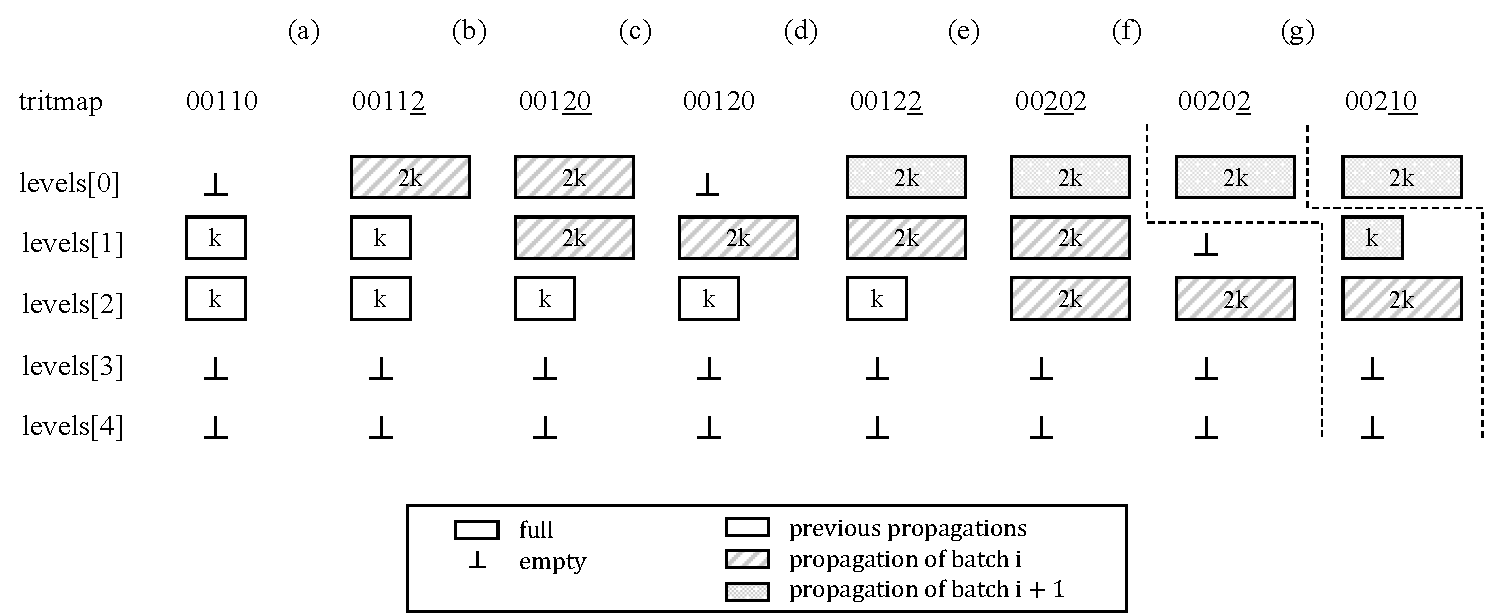
\includegraphics[width=\textwidth,trim={0 0cm 0 0},clip]{graphics/algorithm/propagate_short.pdf}
\centering
\captionsetup{justification=centering}
\caption[\mysketch~\xspace propagation.]{\mysketch~\xspace propagation. \par \small \textbf{(a)} The owner of batch $i$, owner($i$), inserts batch $i$ to level $0$ and atomically updates $tritmap[0]$ to $2$. \\
\textbf{(b)} owner($i$) merges level $0$ with level $1$ and changes $tritmap[1,0]$ from $[1,2]$ to $[2,0]$. \\
\textbf{(c)} owner($i$) clears level $0$. \\
\textbf{(d)} owner($i+1$) inserts its batch to level $0$ and atomically updates $tritmap[0]$ to $2$. \\
\textbf{(e)} owner($i$) merges level $1$ with level $2$, and sets $tritmap[2,1]$ to $[2,0]$. Batch $i+1$ is still blocked because level $1$ has not been cleared yet. \\
\textbf{(f)} owner($i$) clears level $1$. \\
\textbf{(g)} Now owner($i+1$) successfully merges level $0$ with the empty level $1$, and sets $tritmap[1,0]$ to $[1,0]$. 
}
\label{fig: propagate}
\end{figure*}

%============================================================
\section{Query} \label{sec:query_alg} %cached atomic snapshot
%============================================================

% To simplify the query presentation we first present a one-time query and discuss its correctness. We then explain how our caching mechanism works. 

Queries are performed by an unbounded number of query threads. A query returns an approximation based on a subset of the stream processed so far including all elements whose propagation into the levels array begun before the query was invoked. The query is served from an atomic snapshot of the levels array. The pseudo-code is presented in Algorithm~\ref{alg:sl_query}. Instead of collecting a new snapshot for each query, we cache the snapshot so that queries may be serviced from this cache, as long as the snapshot isn't too stale. The snapshot and the tritmap value that represents it are cached in local variables, $\mathit{snapshot}$ and $\mathit{myTrit}$, respectively. Query freshness is controlled by the parameter $\rho$, which bounds the ratio between the current stream size and the cached stream size. As long as this threshold is not exceeded, the cached snapshot may be returned (Lines~\ref{Line:check_rho}-\ref{Line:query_from_cache}). Otherwise, a new snapshot is taken and cached. 
%Our implementation is strongly linearizable, with a formal proof is given in the \fcolorbox{red}{yellow}{Appendix}. Query results are approximate but within well defined error bounds that are user configurable by trading off sketch size, and the error analysis is presented in Section~\ref{sec:analysis}.


The snapshot is obtained by first reading the tritmap, then reading the levels from $0$ to $MAX\_LEVEL$, and then reading the tritmap again. If both reads of the tritmap represent the same stream size then they represent the same stream. We can use the levels read to reconstruct some state that represents this stream. The process is repeated until two such tritmap values are read. For example, focusing on the last two phases of the propagation in Figure~\ref{fig: propagate}, lets assume a query thread $T_q$ reads $tm1=00202$, then reads the levels from $\mathit{levels[0]}$ to $\mathit{levels[4]}$ as depicted in Figure~\ref{fig: propagate} (between the dashed lines), and then read $tm2=00210$. The two tritmap reads represent the same stream of size $10k$, thus a snapshot representing the same stream can be constructed from the levels read. The pseudo-code for calculating the stream size is presented in Algorithm~\ref{alg:tritmap}. Each level is read atomically as the levels arrays are immutable and replaced by pointer swings. The snapshot is a subset of the levels summarizing the stream. To construct the snapshot, the collected levels are iterated over, in reversed order, from $\mathit{MAX\_LEVEL}$ to $0$, and level $i$ is added to the snapshot only if the total collected stream size (including level $i$) is less than or equal to the stream size represented by the tritmap (Line~\ref{Line:add_to_snapshot}). Back to our last example, the size of each level collected by $T_q$ is ${2k,k,2k,0,0}$ (in descending order). As explained, to construct the snapshot, we go over the collected levels from $\mathit{snapLevels[4]}$ to $\mathit{snapLevels[0]}$. By reading $snapLevels[1]$, the total stream size represented by snapshot is $0+0+4\cdot2k+2\cdot k = 10k$. As the stream size represented by $tm1$ and $tm2$ is $10k$, the construction of the snapshot is done and all elements of the processed stream are represented exactly once. The tritmap $\mathit{myTrit}$ maintains the total size of the collected stream and each trit describes the state of a collected level. If level i was collected to the snapshot, the value of $\mathit{myTrit[i]}$ is the size of level i divided by $k$ (Line~\ref{Line:update_myTrit}). 

 
\begin{algorithm}[h]
\caption{Tritmap} \label{alg:tritmap}
\begin{algorithmic}
\setcounter{ALG@line}{\value{mycounter}}
\Procedure{streamSize}{}
        \State \myvar{curr\_stream} $\gets$ 0
        \For{\myvar{i} $\gets$ $0,\dots,\mathit{MAX\_LEVEL}$}
            \State \myvar{weight} $\gets 2^i $
            \If{\myvar{tritmap}[\myvar{i}] $=1$}
                \State \myvar{curr\_stream} $\gets$ \myvar{curr\_stream} $+$ \myvar{weight}$\cdot k$
            \ElsIf{\myvar{tritmap}[\myvar{i}] $=2$}
                     \State \myvar{curr\_stream} $\gets$ \myvar{curr\_stream} $+$ \myvar{weight}$\cdot 2k$
            \EndIf
        \EndFor
        \State \Return{\myvar{curr\_stream}}
\EndProcedure
\setcounter{mycounter}{\value{ALG@line}}
\end{algorithmic}
\end{algorithm}
 
 
\begin{algorithm}[h]
\caption{Query} \label{alg:sl_query}
\begin{algorithmic}
\setcounter{ALG@line}{\value{mycounter}}
\Procedure{Query}{$\phi$}
    \State \myvar{tm1} $\gets$ tritmap \label{Line:read_current_stream}
    \If{$\frac{tm1.streamSize()}{myTrit.streamSize()}$ $\leq$  $\rho$} \label{Line:check_rho}
        \State \Return{snapshot.query($\phi$)} \label{Line:query_from_cache}
    \EndIf
    \Repeat \label{Line:start_collect_levels}
        \State \myvar{tm1} $\gets$ tritmap
        \State \myvar{snapLevels} $\gets$ read \myvar{levels} $0$ to \myvar{MAX\_LEVEL} \label{Line: read_snap}
        \State \myvar{tm2} $\gets$ \myvar{tritmap} \label{Line: second-collect}
    \Until{\myvar{tm1}.streamSize() = \myvar{tm2}.streamSize() }  \label{Line:query_linearization}
    \State \myvar{myTrit} $\gets 0$ \label{line: query_estimate_start}
    \State \myvar{snapshot} $\gets$ empty \myvar{snapshot}
    \For{\myvar{i} $\gets$ $\mathit{MAX\_LEVEL},\dots,0$} \label{Line:start_collect_snapshot}
        \State \myvar{weight} $\gets 2^i $
        \If{\myvar{snapLevels}[\myvar{i}].size()$\cdot$\myvar{weight}+ \myvar{myTrit}.streamSize()$\leq$\myvar{tm1}.streamSize()} \label{Line:add_to_snapshot}
            \State add \myvar{snapLevels}$[i]$ to \myvar{snapshot} \label{Line:add_level_to_snapshot}
            \State \myvar{myTrit}[\myvar{i}] $\gets$ \myvar{snapLevels}[\myvar{i}].size()$ / k$  \label{Line:update_myTrit} \label{line: query_estimate_end}
            \If{\myvar{myTrit}.streamSize()=\myvar{tm1}.streamSize()} \label{Line:snapshot_done}
                \State \textbf{break}
            \EndIf
        \EndIf
    \EndFor
    \State \Return{\myvar{snapshot}.query($\phi$)} \label{Line:query_result}
\EndProcedure
\setcounter{mycounter}{\value{ALG@line}}
\end{algorithmic}
\end{algorithm}


%As levels propagate from lowest to highest, by reading the levels in the same direction, elements may be read more than once, but no element can be missed. 
As levels propagate from lowest to highest, reading the levels in the same direction ensures that no element would be missed but may cause elements to be represented more than once. Building the snapshot highest to lowest ensures that each element will be accounted once. 
In other words, reading the levels from lowest to highest and building the snapshot highest to lowest ensures that an atomic snapshot is collected, as proven in the following section. 


% Queries are performed by an unbounded number of query threads. Instead of collecting a new snapshot for each query, we cache the snapshot so that queries may be serviced from this cache, as long as the snapshot isn't too stale. Query freshness is controlled by the parameter $\rho$, which bounds the ratio between the current stream size and the cached stream size.
% Let $n_{old}$ be the stream size of the cached snapshot, and let $n_{new}$ be the current stream size.
% As long as this threshold is not exceeded ($n_{new} / n_{old} \leq \rho$), the cached snapshot may be returned (Lines~\ref{Line:check_rho}-\ref{Line:query_from_cache}). Otherwise, a new snapshot is taken and cached. 
%after which the thread's cached snapshot is considered invalid and must be rebuilt (Lines~\ref{Line: read_current_stream}-\ref{Line: query_from_cache}).
%Let $n_{old}$ be the stream size of the cached snapshot, and let $n_{new}$ be the current stream size. If $n_{new} / n_{old} \leq \rho$ then the query is answered from the cached snapshot. Otherwise, or if no snapshot is cached, a strongly linearizable snapshot is taken. Once a new snapshot has been built, it is cached.

%============================================================
\subsection{Query's Snapshot Correctness}
%============================================================
Let $\sigma$ be an execution of \mysketch and let $tm1$ and $tm2$ be responses of two read operations of $tritmap$, $op_1$ and $op_2$, respectively, in $\sigma$, such that $op_1$ precedes $op_2$. Let $\mathnormal{A}$ be the stream represented by $tm1$. We will prove that the constructed \emph{snapshot} in Algorithm~\ref{alg: sl_query}, Lines~\ref{line: query_estimate_start}-\ref{line: query_estimate_end}, summarizes the same stream $\mathnormal{A}$. We denote by $|\mathnormal{A}|$ to be the stream size and by $|snapshot|$ to be the size of the stream currently represented by $snapshot$.
Let \emph{snapLevels} be the set all levels read between $op_1$ and $op_2$.

First, we show that $tm1$ and $tm2$ represent the same stream, i.e.  $\mathnormal{A}$.

\begin{lemma}
Let $tm1$ and $tm2$ be responses of two read operations of $tritmap$.
If $tm1$ and $tm2$ represent streams with equal size then $tm1$ and $tm2$ represent the same stream.
\end{lemma}
\begin{proof}
By definition the variable tritmap is 3-based, 31 digits non-negative integer that is atomically updated by DCAS operation and is only increasing.   
\end{proof}

Second, we show that $snapLevels$ contains all sampled elements in the sketch, immediately after $tm2$, summarizing the stream $\mathnormal{A}$.

\begin{lemma}\label{Lem: snap_no_miss}
The set of levels, $snapLevels$, read between the two \emph{tritmap}'s reads, $op_1$ and $op_2$, contains all sampled elements summarizing the stream $\mathnormal{A}$.
\end{lemma}
\begin{proof}
Let $x$ be an element in level $j$ immediately after $tm1$.
If $x$ exists in level $j$ during the read of sketch's levels in Algorithm~\ref{alg: sl_query} Line~\ref{Line: read_snap}, then we are done.
Otherwise, a propagation occurred in between the reads such that level $j$ was merged with the next level and cleared. During this merge, all level $j$'s elements, including $x$, were sampled and propagated to level $j+1$. If $x$ exists in level $j+1$ in the set $snapLevels$ then we are done, if not, we apply the above argument again. This continues up to MAX\_LEVEL and therefore snap contains the element $x$.
\end{proof}

The following refers to the construction of the subset \emph{snapshot} from level MAX\_LEVEL to 0:

\begin{lemma} \label{Lem: all_dup}
If level $j$ contains an element represented by the snapshot thus far, all elements in level $j$ are also (already) represented by this snapshot.
\end{lemma}
\begin{proof}
During a call to the procedure \emph{propagate} with level $j$, the elements in that level are sampled and merged with level $j+1$, resulting in level $j+1$ representing also the elements of (former) level $j$.
Let $x$ be an element represented by level $j$ in the set $snapLevels$.
$x$ is also represented by level $i$ such that level $i$ is in the current \emph{snapshot} and $i>j$. Consider the process of propagation from level $j$ to level $i$, it follows from the above that level $i$ also represents all the elements in level $j$.
\end{proof}

Each element in level $j$ represents $2^i$ elements from the processed stream.

\begin{lemma}\label{Lem: all_in_no_dup}
If level $j$ represents new elements that are not represented by snapshot, the size of the sub-stream left to represent is at least the size of the representation of level $j$.

If level $j$ represents elements already represented by snapshot, the sub-stream left to represent is smaller than the representation of level $j$.
\end{lemma}
\begin{proof}
We will prove the first part by contradiction. Assume by contradiction that the size of sub-stream left to represent is smaller than the size of the representation of level $j$ such that $|snapshot\cup level[j]| > |\mathnormal{A}|$. It follows from Lemma~\ref{Lem: snap_no_miss} that level $j$ contains at least one duplicated element (an element already represented by level $i$ in \emph{snapshot} such that $i>j$). From Lemma~\ref{Lem: all_dup} all level $j$'s elements are duplicated and already being represented by the current \emph{snapshot}. Contradiction. 

Now, for the second part, assume that an element $x$ is represented more than once by the current \emph{snapshot}. Let level $j$ be the second level to be added to \emph{snapshot} that also represents $x$ (first time to duplicate the representation of $x$). From Lemma~\ref{Lem: all_dup}, all elements in level $j$ are already represented by this snapshot.
If level $j$ contains $2k$ elements, the size of sub-stream represented by level $j$ is $2k\cdot2^j$, and the size of the sub-stream left to represent is at most represented by levels 0 to $j-1$, meaning the size is at most $2k(1+2+\dots+2^{j-1})=2k(2^j-1)$ which is smaller than the size of sub-stream represented by level $j$.
If level $j$ contains $k$ elements and is already represented by level $i$, $i>j$, in \emph{snapshot}, level $j-1$ must have propagated level $j$ deeper, i.e. level $j-1$ is also represented by level $i$, therefore, also already represented by \emph{snapshot}. Level $j$ represents $k\cdot2^j$. The size of the sub-stream left to represent is at most represented by levels 0 to $j-2$, meaning the size is at most $2k(1+2+\dots+2^{j-2})=k(2^{j-1}-2)$, which is smaller than the size of sub-stream represented by level $j$.
\end{proof}


\begin{lemma} \label{Lem: query_estimate}
The snapshot constructed in Algorithm~\ref{alg: sl_query}, Lines~\ref{line: query_estimate_start}-\ref{line: query_estimate_end}, summarizes the same stream, $\mathnormal{A}$, as represented by the second tritmap read, $tm2$, in Algorithm~\ref{alg: sl_query}, Line~\ref{Line: second-collect}. 
\end{lemma}
\begin{proof}
From Lemma~\ref{Lem: all_in_no_dup} $|snapshot|=|\mathnormal{A}|$ and every element is represented at most once in the constructed \emph{snapshot}.
\end{proof}

